\chapter{SYSTEM DESIGN AND IMPLEMENTATION}
\label{chap:caseFarming}

This chapter describes the proposed solution which is a system consists of two subsystems: A crowd-sourcing system and an analysis system. In \textit{Requirement analysis and System overview} subsection, everything is briefly described as a whole. In two last sections, structure and details of two subsystems are defined more comprehensively.

\section{Requirement analysis and system overview}
\subsection{Requirement analysis}

To be able to utilize data to serve a security purpose, the most obvious method would be to analyze visual data such as photos and videos, and the current most effective way to do so is using Artificial Intelligence. In recent years, advancements in Artificial Intelligence, especially in Neural Networks, significantly enhanced the development of computer vision field. On the famous ImageNet \footnotetext{Source: \url:{http://www.image-net.org/challenges/LSVRC/}} dataset, trained neural networks can now generate results that are better than human in classifying images (Figure \ref{chap3:deeplearning_vs_human}). 

For Deep learning models to be successful, sufficient training data must be provided. \cite{DBLP:journals/corr/SunSSG17} Found out that the effectiveness of computer vision related tasks scales logarithmically with the amount of training data. Regardless of the importance of data in Deep learning models, there are few to none security datasets that are suitable for the environment of Vietnam.     

\begin{center}
    \begin{figure}[H]
    \centering
    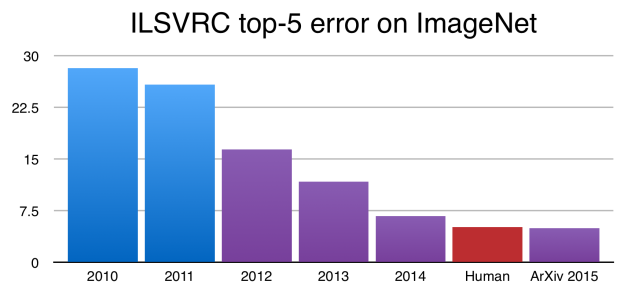
\includegraphics[width=0.75\columnwidth]{images/chap3/deeplearning_vs_human.png}
    \footcaption{Neural Network out-performing human in 2015 on ImageNet Large Scale Visual Recognition Challenge}
    \label{chap3:deeplearning_vs_human}
    \end{figure}
\end{center}
\footnotetext{Source: \url:{ https://devblogs.nvidia.com/mocha-jl-deep-learning-julia/}}

Figure \ref{chap3:system_overview_basic} shows a concise overview of how the system operates. Users interact with the \textbf{Crowd-sourcing system} through \textbf{User Interfaces}. The input of users can come in the form of images, videos or label contribution and are stored in the database. The system is also responsible for obtaining appropriate contents from the database to display to users through user interfaces.

\begin{center}
    \begin{figure}[H]
    \centering
    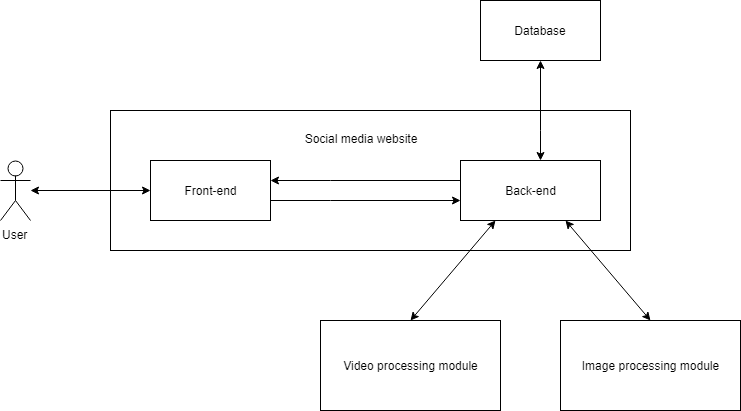
\includegraphics[width=1\columnwidth]{images/chap3/system_overview_basic.png}
    \caption{An overview of the system}
    \label{chap3:system_overview_basic}
    \end{figure}
\end{center}

Whenever there are videos to analyze, the server will send them to the \textbf{Video classifier module}, then get results back. Results returned from video classifier module are classified activity from the video and frames that contain faces in them. \textbf{Face Recognition module} does the job of identifying people in images. Results of both \textbf{Video classifier module} and \textbf{Face Recognition module} are used to determine security threats each video or image shows.
\section{Crowd-sourcing system}
\subsection{Database}
The project database divides into two different parts: \textbf{Cloud storage} and a \textbf{NoSQL database}. The primary target is to reduce website loading time. Let take an example, if files are stored directly on the crowd-sourcing server. When many users request a file simultaneously, the server with limited bandwidth will cause delay. “53\% of mobile site visitors leave a page that takes longer than three seconds to load” – \href{https://think.storage.googleapis.com/docs/mobile-page-speed-new-industry-benchmarks.pdf}{Google}. If these files stored on cloud storage, the client will be served by the cloud storage provider, which has higher availability.
\section{Analysis system}
The project requires two systems for analysis: A face recognition system and a video classifier system. The facial recognition system takes pictures of human faces as input and returns their identification. The video classifier system analyzes videos to find out actions in them. The remaining of this section describes in detail about the two analysis system.
\subsection{Face recognition module}
\subsection{Video classifier module}
Video classifying is not a new task in the field of Deep learning.
	
\section{Technologies}
\subsection{Node.js and npm}
Node.js (Node) is a JavaScript runtime built on Chrome's V8 JavaScript engine (cite). Node supports executing JavaScript on server-side. Ryan Dahl was created Node.js in 2009. Node.js Foundation is in charge of the development of Node.js. After nine years since its release, the latest LTS version of Node.js is 10.14.2 (includes npm 6.4.1). “Node.js operates on a single thread, using non-blocking I/O calls, allowing it to support tens of thousands (cite) of concurrent connections held in the event loop.” Although JavaScript is single-threaded, thanks to the Event loop, Node.js can implement asynchronous I/O operations. The Event loop will transfer operations to the system kernel. “Since most modern kernels are multi-threaded, they can handle multiple operations executing in the background. When one of these operations completes, the kernel tells Node.js so that the appropriate callback may be added to the poll queue to executed eventually”. By utilizes non-blocking I/O, Node.js skips the waiting time for I/O calls, which is much higher than processing time.
\section{Implementation}